<<<<<<< HEAD
%------------------------------------------------
\section{Second Section}
%------------------------------------------------

\begin{frame}
\frametitle{Table}
\begin{table}
\begin{tabular}{l l l}
\toprule
\textbf{Treatments} & \textbf{Response 1} & \textbf{Response 2}\\
\midrule
Treatment 1 & 0.0003262 & 0.562 \\
Treatment 2 & 0.0015681 & 0.910 \\
Treatment 3 & 0.0009271 & 0.296 \\
\bottomrule
\end{tabular}
\caption{Table caption}
\end{table}
\end{frame}

%------------------------------------------------

\begin{frame}
\frametitle{Theorem}
\begin{theorem}[Mass--energy equivalence]
$E = mc^2$
\end{theorem}
\end{frame}

%------------------------------------------------

\begin{frame}[fragile] % Need to use the fragile option when verbatim is used in the slide
\frametitle{Verbatim}
\begin{example}[Theorem Slide Code]
soguvhsqn
\end{example}
\end{frame}

%------------------------------------------------

\begin{frame}
\frametitle{Figure}
Uncomment the code on this slide to include your own image from the same directory as the template .TeX file.
%\begin{figure}
%\includegraphics[width=0.8\linewidth]{test}
%\end{figure}
\end{frame}
=======
% --------------------------------------------------

\begin{frame}
  \frametitle{Parallélisation de Routino}
  \begin{itemize}
  \item Séquentiel par portions
    \vspace{1em}
  \item Utilisation des données des précédentes portions
  \end{itemize}
\end{frame}

% --------------------------------------------------

\begin{frame}
  \frametitle{Parallélisation de Routino}

  \begin{itemize}
  \item Tour de France : En séquentiel
  \end{itemize}

  \begin{center}
    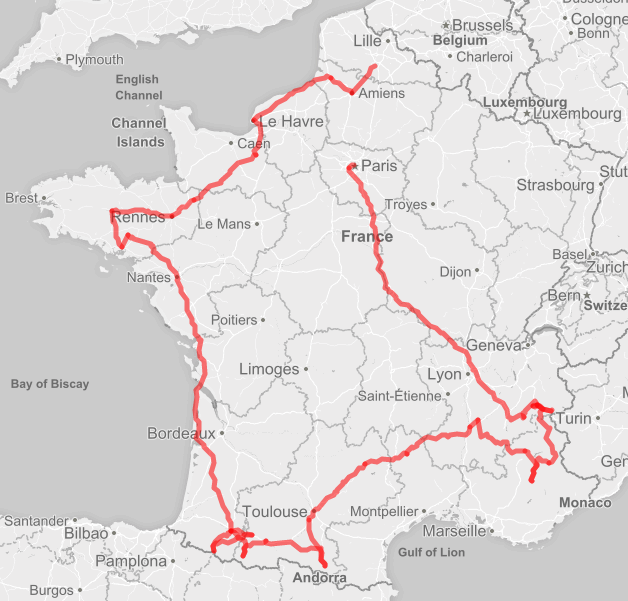
\includegraphics[scale=0.33]{include/tourfrance_mono.png}
  \end{center}

\end{frame}

% --------------------------------------------------

\begin{frame}
  \frametitle{Parallélisation de Routino}
  
  \begin{itemize}
  \item Tour de France : En Multithread
  \end{itemize}

  \begin{center}
    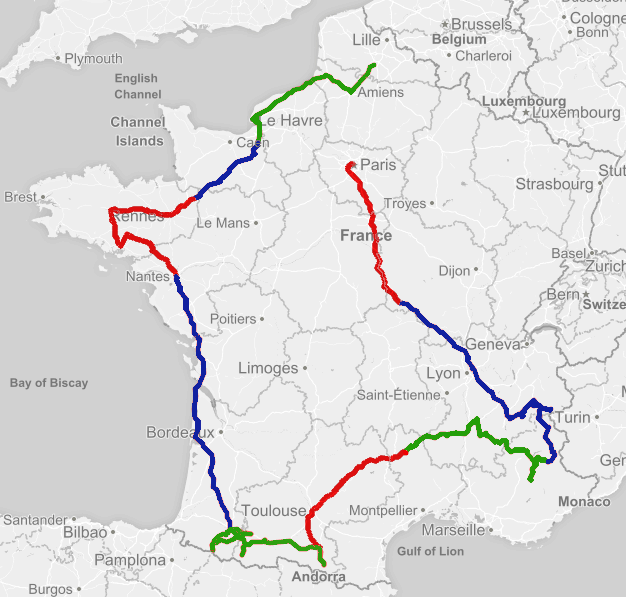
\includegraphics[scale=0.33]{include/tourfrance_multi.png}
  \end{center}
  
\end{frame}

% --------------------------------------------------

\begin{frame}
  \frametitle{Parallélisation de Routino}

  \begin{itemize}
  \item Rendre les portions indépendantes/
    \vspace{1em}
  \item Un minimum de synchronisation
  \end{itemize}

\end{frame}

% --------------------------------------------------

\begin{frame}
  \frametitle{Parallélisation de Routino}

  \begin{center}
    \only<1>{
\includegraphics[scale=0.34]{include/multi1.pdf}}
    \only<2>{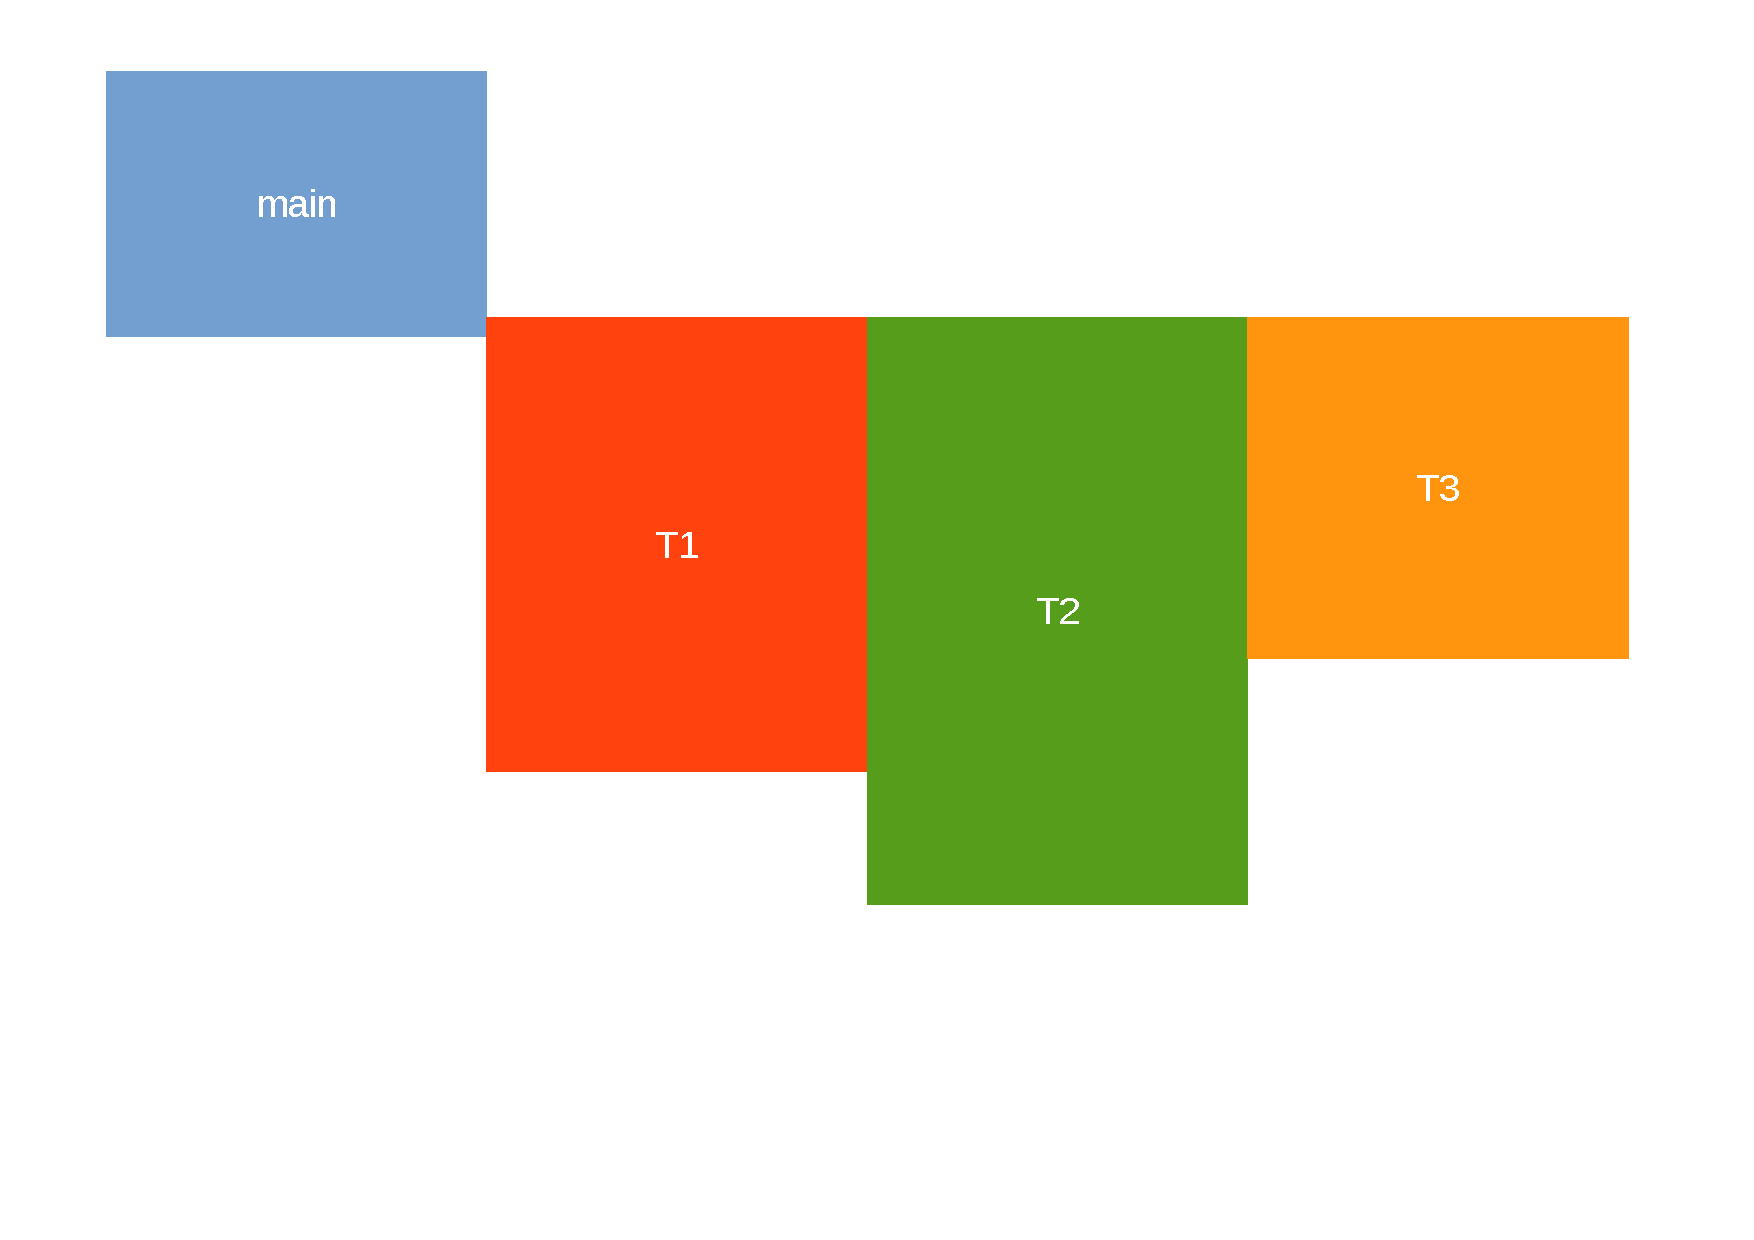
\includegraphics[scale=0.34]{include/multi2.pdf}}
    \only<3>{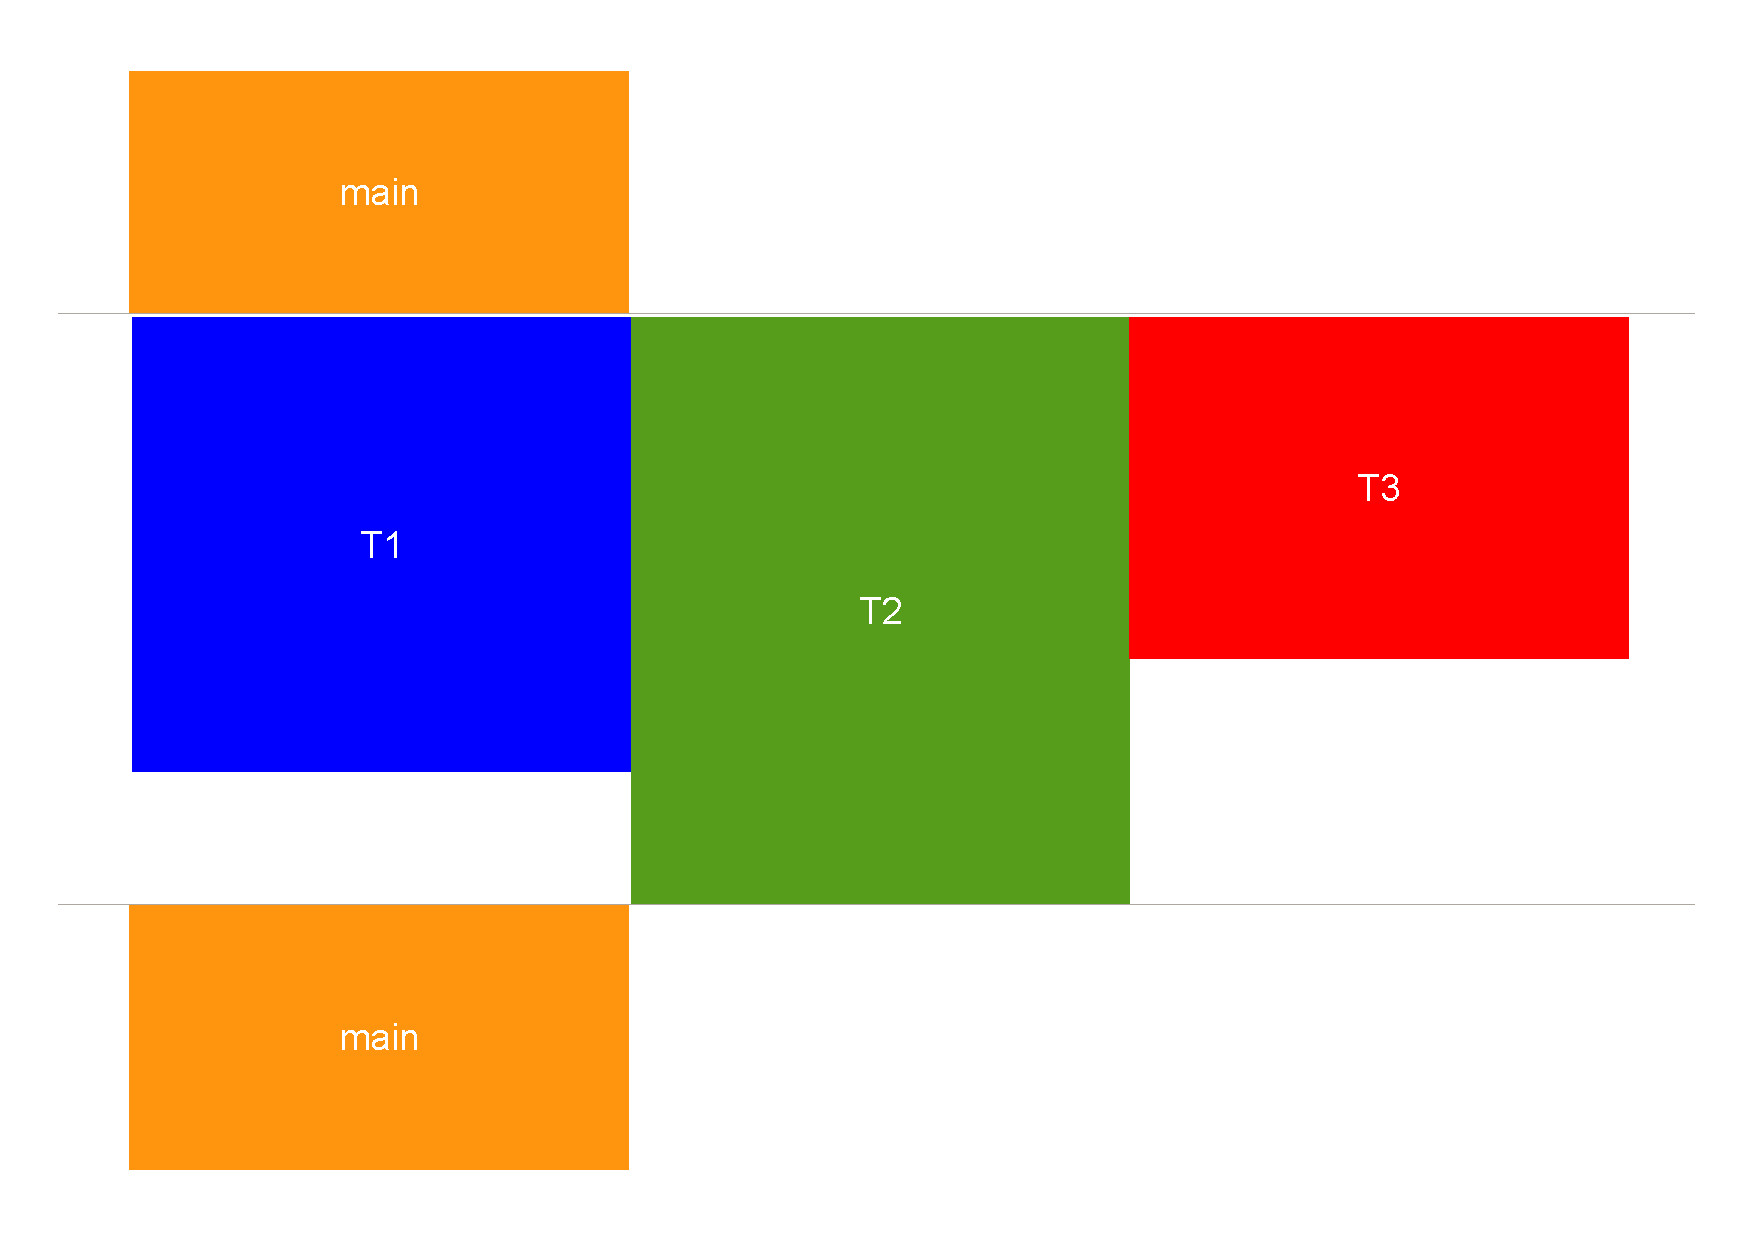
\includegraphics[scale=0.34]{include/multi3.pdf}}
  \end{center}

\end{frame}

% --------------------------------------------------

\begin{frame}
  \frametitle{Evaluation du Multithread}

  \begin{itemize}
  \item Usage CPU
  \end{itemize}

  \begin{center}
    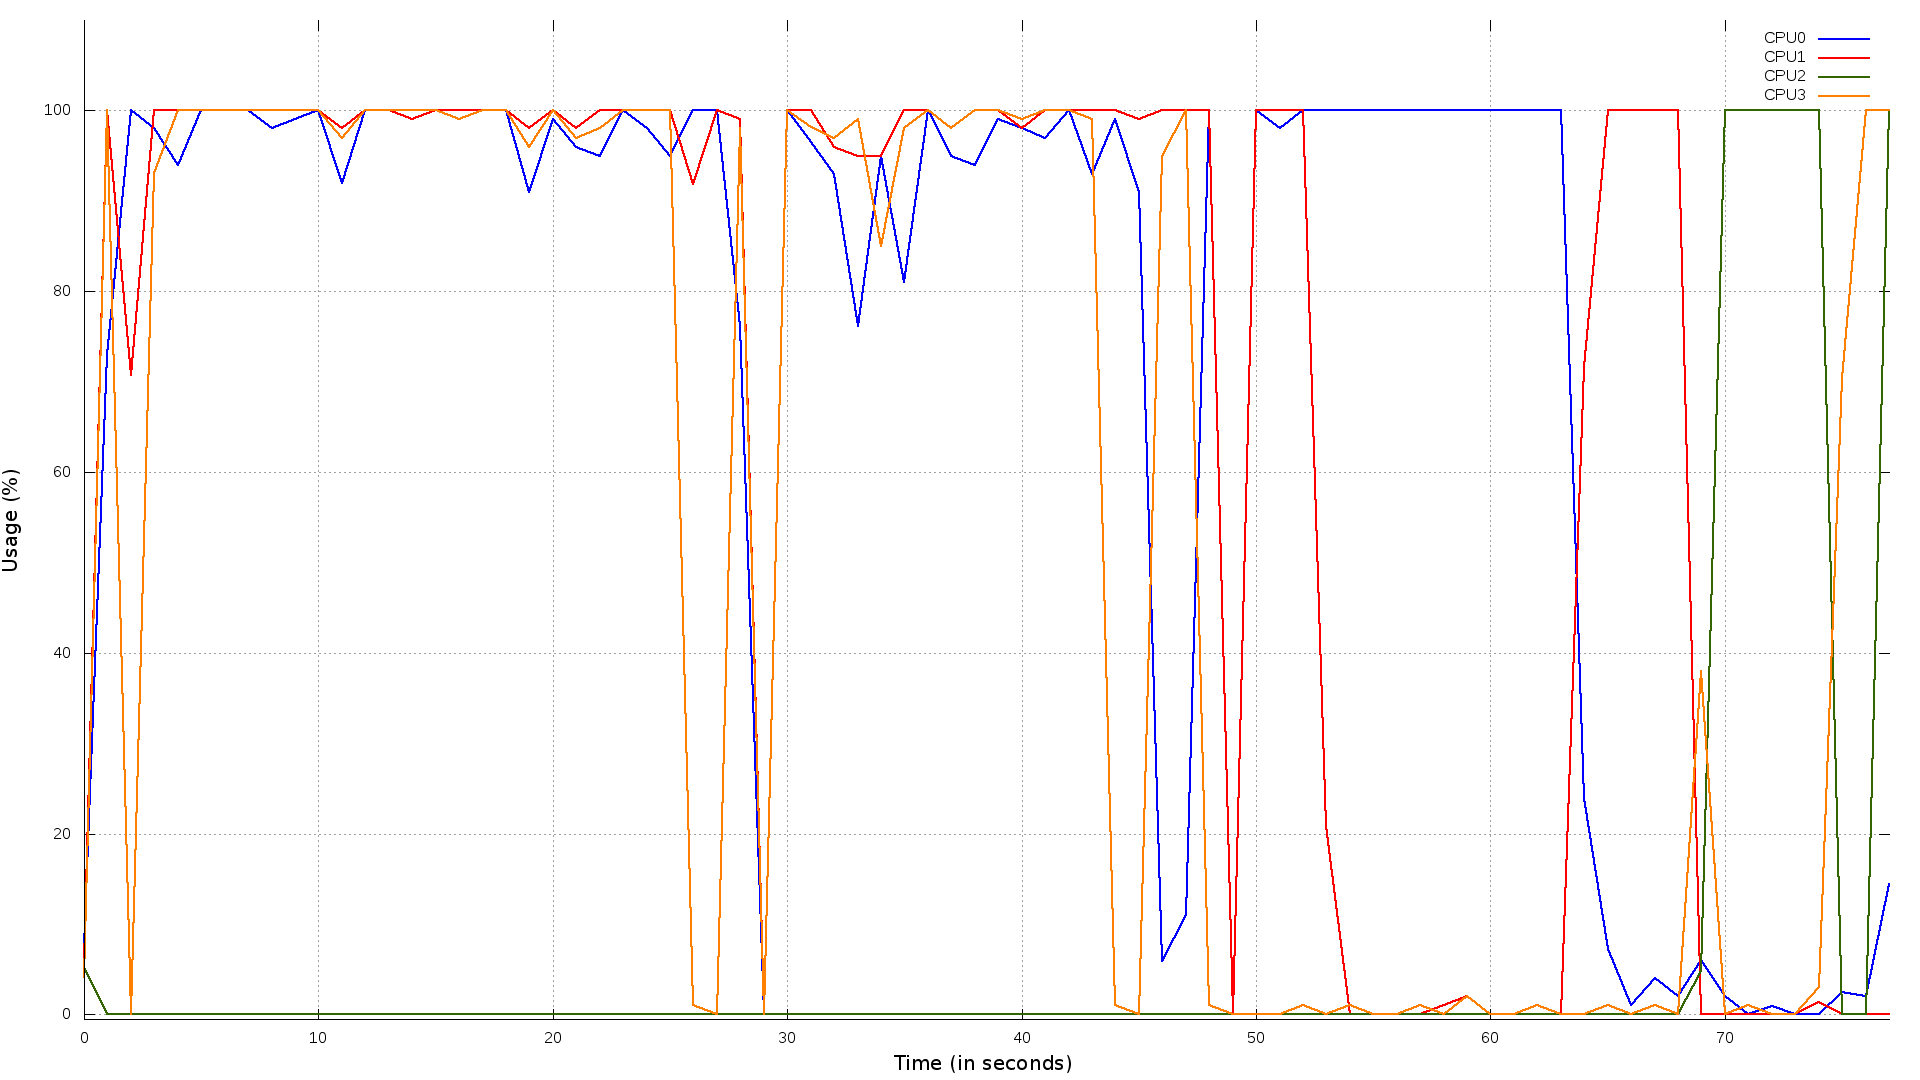
\includegraphics[scale=0.24]{include/cpu_usage.png}
  \end{center}

\end{frame}

% --------------------------------------------------
>>>>>>> d0e4d77a3b88ddd517a0b32941ba2cec9ae915e8
